%%This is a very basic article template.
%%There is just one section and two subsections.
\documentclass[a4paper, 11pt]{scrartcl}
\usepackage{color}
\usepackage{a4wide}
\usepackage[english]{babel}
\usepackage[T1]{fontenc}
\usepackage[utf8]{inputenc}
\usepackage{amsthm,amsfonts,amssymb,amsmath,amsbsy}
\usepackage{ngerman}
\usepackage{amsthm}
\usepackage{graphicx}
\usepackage{listings}
\usepackage{multicol}
\usepackage{color}
\usepackage{subcaption}
\usepackage{multirow}
\usepackage{booktabs}
\usepackage{ifthen}
\usepackage{hyperref}
\usepackage{enumerate}

\usepackage{color}
\definecolor{gray}{rgb}{0.4,0.4,0.4}
\definecolor{darkblue}{rgb}{0.0,0.0,0.6}
\definecolor{cyan}{rgb}{0.0,0.6,0.6}

%%%%%%%%%%%%     FOR XML SYNTAX HIGHLIGHTING     %%%%%%%%%%%%%%
\lstset{
  basicstyle=\ttfamily,
  columns=fullflexible,
  showstringspaces=false,
  commentstyle=\color{gray}\upshape
}

\lstdefinelanguage{XML}
{
  morestring=[b]",
  morestring=[s]{>}{<},
  morecomment=[s]{<?}{?>},
  stringstyle=\color{black},
  identifierstyle=\color{darkblue},
  keywordstyle=\color{cyan},
  morekeywords={xmlns,version,type}% list your attributes here
}
%%%%%%%%%%%%%%%%%%%%%%%%%%%%%%%%%%%%%%%%%%%

%%% A custom enviroment %%%
%% Use
% \begin{numerate}[ABC]
% \item[opt-header] ...
%% to use the environment.
%% It generates a list numerated in the style /ABC010/ <opt-header>\\, /ABC020/ <opt-header>\\, ...
%\newcommand{\mylabel}[1]{
%    \ifcsname c@#1\endcsname%
%    \else%
%        \newcounter{#1}\label{#1}%
%    \fi%
%}
\makeatletter
%\newcommand{\mylabell}[1]{
%    \@ifundefined{r@#1}{\label{#1}}{X}
%}
\newenvironment{numerate}[1][]{% The  \begin{numerate}  replacement
	\begin{enumerate}

	\newcommand{\numerateName}{#1}

	% If the counter with this name has not be defined before
	\@ifundefined{c@numerate_counter_#1}{
		% Create it
		\newcounter{numerate_counter_#1}
		\setcounter{enumi}{9}
	}{
		% Else countinue the counting with the old value
		\setcounter{enumi}{\value{numerate_counter_#1}}
	}

	% Move the captions to the right
	% Move it for a fixed value to the right => Different captions start at different positions
	\setlength{\itemindent}{1.5cm}

	% Create the number
	\renewcommand{\labelenumi}
		{\textbf{/#1\ifnum\value{enumi}<100 0\fi \ifnum\value{enumi}<10 0\fi \theenumi/}}

	% Move it for the captionlength to the right: They start directly above their text bodies
	%\settowidth{\itemindent}{\labelenumi}

	\let\olditem\item
	% Create the titel, if any
	\renewcommand{\item}[1][]
		{\olditem \addtocounter{enumi}{9} % Draw the counter and increment it
% A try on labels
%			\ifthenelse{\equal{##2}{}} % If a label-parameter is NOT given...
%				{
%					\ifthenelse{\equal{##1}{}} % If not, check if there is a describtion
%						{\label{#1\theenumi}} % If there is no description, use the number as label
%						{\label{##1}} % If there is a description, use it as label
%				}
%				{\label{##2}} % If the label-parameter is given, use it
			\ifthenelse{\equal{##1}{}}{}{\space\textbf{##1}\\} % Print the given description
			}
} { % The  \end{numerate}  replacement
	\setcounter{numerate_counter_\numerateName}{\value{enumi}}
	\end{enumerate}
}
\makeatother

\hypersetup{
	colorlinks,
	citecolor = black,
	filecolor = black,
	linkcolor = black,
	urlcolor = black
}

\usepackage{geometry}
\geometry{a4paper,left=20mm,right=20mm, top=2cm, bottom=3cm}

\author{Vincent Diener, Kenan Ibrahimov,\\ 
        Sebastian Friebe, Sarah Lutteropp,\\ 
        Melanie Magin, Kris Reiling}
\title{%\vspace{1cm}
         
\includegraphics[scale=1.3, angle=270]{../logo.pdf}\\
         \vspace{5mm}
         Campus Location and Navigation
         \vspace{5mm}}
\subtitle{Functional Specifications Document}
\date{\today}

\newcommand{\programName}{\textit{CLAN}}

\setcounter{tocdepth}{2} % hide subsubsections in table of contents

\begin{document}

\maketitle
\thispagestyle{empty}

\newpage

\pagenumbering{roman}
\tableofcontents

\newpage

\pagenumbering{arabic}

\section{Introduction}

It is often difficult for KIT visitors and new students to find the buildings, rooms or the ways between them on the campus. Our product will simplify this task, leading to better time efficiency and less stress for everyone.

The general goal of this project is the design and implementation of a routing system for the KIT campus. The system will be able to compute and to display the shortest path between a starting point and a destination. It will be possible to route from and to buildings and rooms inside buildings. For the latter, the system will display a floor plan map of the building. It will also be possible to search just for the destination, without computing a route from some other point. \\

\noindent On the administration side, the system will provide a graphical use interface (\textit{GUI}) to modify the routing graph if needed (in case of construction works or if some more details are needed) or create it from scratch. It will be possible to easily add/delete buildings with or without routing information of the interior. Moreover, it will be possible to add vertices and edges with information that is necessary to do the routing.

The product will be shipped with \textit{floor plan maps} of at least two buildings of ``KIT Campus Süd'' and a \textit{map} of the campus exterior.


%Both routing and administration will share a component for map visualization.

%\subsection{Routing}
%
%The routing starts with the user input. It will be easy for the user to specify a building, a room or a lecture hall as starting point or destination. The system will compute a shortest path from the starting point to the destination. The methods of user interaction are more closely described in the mandatory criteria section of this document. \\
%
%\subsection{Map Data - Administration Tool}
%
%Administration tool will be used to create the map data. It will be possible to add and edit every piece of data that is or can be used by the routing application. The functionality of the administration tool is described
%in detail in the mandatory criteria section of this document.

\section{Objectives}


In this section, we describe in detail the features of the routing tool and the admin tool. This includes the functionality and the different ways for the user to input data into the tools, as well as how the
tools process that information and shows it to the user.

\subsection{Mandatory Criteria -- Routing Tool} %Searching \& Routing}

\paragraph{Displaying the map}
\begin{itemize}
	\item An exterior \textit{map} of the campus is displayed. % without the underlying graph
%		\begin{addmargin}[7mm]{0mm}
%			It is possible to just look at the map of the campus, without searching for any points or routes.
%		\end{addmargin}
	\item Interior \textit{floor plan maps} can be displayed.
		\begin{addmargin}[7mm]{0mm}
		Apart from showing the campus \textit{map}, the system is also capable of displaying the \textit{floor plan map} of a building. %However, at each point in time only one map (i.e. either a floor plan map or the exterior map) is displayed.
		\end{addmargin}

	\item Stairs can be displayed.
		\begin{addmargin}[7mm]{0mm}
		If the route contains stairs, they will be displayed as an arrow pointing upwards or downwards.
		\end{addmargin}

	\item If the user searches for a location, it is highlighted on the \textit{map}.
	\item Ways passing under/through buildings are displayed in another color.
\end{itemize}

\paragraph{Navigation in the map}
\begin{itemize}
	\item The user can change his viewpoint by zooming in/out and panning.
	\item The user can enter a building, switch between floors and leave a building.
		\begin{addmargin}[7mm]{0mm}
			When selecting a building, the ground \textit{floor plan map} of the selected building will be displayed. Once this happens, it is possible for the user to switch between the different floors of the selected building and leave the building again.
		\end{addmargin}
\end{itemize}

\paragraph{User input}
\begin{itemize}
	\item The user can search for a location.
		\begin{addmargin}[7mm]{0mm}
			Locations can be searched for by entering identifying information. This information includes building names and numbers, room names and addresses.
			%By using these text fields, the user can provide a start and end point when searching for a route.
		\end{addmargin}
	\item The user can search for a route.
		\begin{addmargin}[7mm]{0mm}
			The user can provide a start and end point for searching a route between them.
		\end{addmargin}
	\item Search suggestions (auto-completion) are provided in the \textit{search fields}.
	\item Start and destination for routing can be selected by clicking on the \textit{map}.
\end{itemize}

\paragraph{Computing the route}
\begin{itemize}
	\item The shortest path between two locations (in- and outdoor) is computed.
		\begin{addmargin}[7mm]{0mm}
			It is possible to search for routes on the whole campus \textit{map}. Those routes may or may not start or end in buildings.
		\end{addmargin}
	%\item Find a location
	\item Routing for pedestrians is provided.
	\item A fast algorithm is used for routing.
		\begin{addmargin}[7mm]{0mm}
			 For further explanation, see ``Nonfunctional Requirements''.
			%Calculation speed is essential for routing applications. Our goal is to minimize this time as much as possible.
		\end{addmargin}
		\item Shortcuts through other buildings are considered.
		\begin{addmargin}[7mm]{0mm}
			 When computing shortest path, the system will take into account routes that pass through other buildings.
		\end{addmargin}
	\item When routing to a building (or lecture hall) with more than one entrance, the path to the nearest entrance is calculated instead of the path to the main entrance.
%	\item The default metric for the computing of the shortest path is constant pedestrian walking speed. (? Move to Product Functionalities?)
\end{itemize}



\paragraph{Output}
\begin{itemize}
	\item A path between two places can be displayed.
		\begin{addmargin}[7mm]{0mm}
			After the user has specified a start and end point, the calculated route is shown on the \textit{map}. The route will be clearly visualized and easy to understand.
		\end{addmargin}
	\item Textbased route output is provided.
		\begin{addmargin}[7mm]{0mm}
			Show a written form of the route. E.g., ``Walk for 100m. Turn right. Walk for 25m. You have reached your destination.'' % Thank you for routing with KIT Campus Navigation.
		\end{addmargin}
\end{itemize}

\subsection{Mandatory Criteria -- Administration Tool}

\paragraph{Modifying the map}
The \textit{map} will be displayed in the same way as in the routing tool and the navigation in it (e.g. zooming, panning) is also the same. There are the following additional features:

\begin{itemize}
	\item The \textit{routing graph} is displayed on top of the \textit{map}.
	\item A set of vertices and edges can be highlighted.
		\begin{addmargin}[7mm]{0mm}
			Vertices and edges of the \textit{routing graph} will be drawn in another color when selected with the mouse.
		\end{addmargin}
	\item The outline of a building can be highlighted. %(TODO: An outline of a building have also to be stored as a polygon path)
		\begin{addmargin}[7mm]{0mm}
			The outline of a building will be drawn in another color when selected with the mouse.
		\end{addmargin}
\end{itemize}

\begin{itemize}
	\item The administrator can create, open and save a \textit{map}.
		\begin{addmargin}[7mm]{0mm}
			It is possible to open and save a \textit{map} of the campus or a \textit{floor plan map} of a building and its underlying \textit{routing graph}.
		\end{addmargin}
	\item The \textit{background image} of the \textit{map} can be exchanged.
	\item Buildings, vertices and edges can be added to or removed from a \textit{map}.
	\item Vertices can be moved and edges can be modified on the \textit{map}.
	\item \textit{Properties} attached to buildings, vertices and edges can be edited.
		\begin{addmargin}[7mm]{0mm}
			These \textit{properties} include for vertices: Name, address, building number and it's entrance. And for edges: Contains stairs (needed for wheelchair users) and opening hours.
		\end{addmargin}
	\item \textit{Floor plan maps} can be added to a building. For example, if you want to add a building with multiple floors, they can be added one after another witch an attached \textit{routing graph}.
	%\item The administrator can add entrances to a building. This information is saved as vertex \textit{property}.

	\item The administrator can add edges representing links between different floors of a building (e.g. stairs, elevators).

	%\item Create links between vertices of different maps
		%\begin{addmargin}[7mm]{0mm}
		%	In order to store maps seperately and connect them with each other, vertices on different maps will be identified with each other by linking them. I.e., it is possible to split the map of the whole campus into smaller maps and put them together.% ( TODO: Maybe it will be helpful to show two maps at the same time in the GUI in order to select the vertices identified with each other?)
		%\end{addmargin}
%	\item Store data in a XML format (? -> Product Data)
\end{itemize}

\subsection{Facultative Criteria -- Routing Tool}

\paragraph{Filtering}
By filtering nodes and edges, we can restrict our \textit{routing graph} to a subgraph of it (e.g. a \textit{graph} that uses no edges with the \textit{property} ``contains stairs''). This will allow for the following additional modes:

\begin{itemize}
	\item Routing for wheelchair users is provided. %(stairs property needed)
	\item Routing for cyclists is provided.
	\item It is possible to search only inside a building.
		\begin{addmargin}[7mm]{0mm}
			It is possible to search for routes within certain buildings only.
		\end{addmargin}
	\item The user can search for points of interest.
		\begin{addmargin}[7mm]{0mm}
			It is possible to search for certain places within buildings, (e.g. locate restrooms inside a building)
			as well as to search for points of interest outside of buildings (e.g. locate bicycle stands on the \textit{map}).
		\end{addmargin}
\end{itemize}

\paragraph{Searching}
\begin{itemize}
	\item When the user types in the \textit{search fields}, spellchecking (using all possible locations as dictionary) is done. %(with Levenshtein distance) (?)
	\item The user can bookmark favourite search requests.
\end{itemize}

\paragraph{Computing the routes}
\begin{itemize}
	\item The user can enter his own average speed to obtain the calculated time needed to walk the route.
	\item The routing destination can be one of multiple places (e.g. nearest restroom, bicycle stand, coffee machine or exit).
\end{itemize}

\paragraph{Android App}
\begin{itemize}
	\item An Android app is provided.
	\item The tool can use \textit{GPS} positions to find the nearest vertex in the underlying \textit{routing graph} of the exterior \textit{map}.
	\item Live routing on a smartphone or tablet with \textit{GPS} is provided.
\end{itemize}

\paragraph{Java Applet}
\begin{itemize}
	\item A Java Applet is provided.
\end{itemize}

\subsection{Facultative Criteria -- Administration Tool}

\begin{itemize}
	%\item Display additional information of vertices and edges in a separate area of the GUI (? -> GUI)
	\item The user of the administration tool can define his own set of filters for routing.
	\item New categories of \textit{properties} (e.g. ``coffee machine'') can be added.
	\item It is possible to close some roads temporarily (e.g. roads that are under construction).
\end{itemize}

\subsection{Excluded Criteria -- Routing Tool}

\begin{itemize}
	\item No routing for cars will be provided.
	\item No \textit{map} data outside ``KIT Campus Süd'' will be provided by the project.
	\item Speech input will not be supported.
	\item Public transportation will not be considered when calculating the route.
	\item No photos of locations/places will be provided.
	\item No alternative routes will be calculated or shown.
	\item The tool is not a server based application.
\end{itemize}

\subsection{Excluded Criteria -- Administration Tool}

\begin{itemize}
	\item There will be no auto generation of the \textit{routing graph} for a \textit{map} from images.
	%\item It is not possible to do freehand drawings on the map. %This is not MS Paint.
	\item No functionality to import/export OpenStreetMap data will be provided.
\end{itemize}


\section{Product Usage}
This section describes how and by whom the product will be used and what they need to use it.
As they share a lot of their functionalities, the routing tool and the administration tool will be implemented within the same application. This allows
the user of the administration tool to switch to the routing tool at any time to test the map he just created.

\subsection{Routing}
\paragraph{Scopes}
Nowadays, it is not unusual for universities to be situated within extensive campuses. While this is of course convenient, it can also be
quite confusing for students, especially for freshmen. They have to look up lecture halls on big, confusing plans that are often not even up to date.
As a result, a lot of time is wasted. We seek to change this with our campus routing tool. The tool provides a well-arranged, simple yet powerful
map application that can be intuitively used by students or people working on the campus to easily find any building or calculate the shortest
route between any two points. The location or route is then visualized in a way that enables users to fully understand where they are or where they are
supposed to go with just one quick look.

\paragraph{Target Audiences}
As mentioned above, the main target audience for the routing application are university students, with the focus being on the students who are new to
the campus. No previous knowledge is needed to use it, so everyone who knows how to use a computer and has access to one will also be able to navigate
with the routing tool. Another target audience is the people working on the campus such as professors, security and cleaning personnel. They might as
well have problems finding their way on the campus when they start to work there.

\subsection{Administration Tool}
\paragraph{Scopes}
The administration tool is used to create the \textit{map} that the routing tool uses. It allows to create it from scratch or modify all the data that is
shown by the routing tool. This includes loading a \textit{background image}, creating the corresponding \textit{routing graph} and adding information to its vertices and edges.
The main goal of the administration tool is to make this difficult, tedious task simple and quick by providing an intuitive interface and automating
many of the time-consuming steps. For example, when adding the building number to one vertex of a building outline, all other vertices will automatically
receive this \textit{property} as well.

\paragraph{Target Audiences}
The \textit{map} will most likely be provided by the universities for their students. Thus, the target audience for the administration tool are people
working for the university. While the tool is mainly self-explanatory, it is also very versatile. The \textit{routing graph} can be edited in a lot of ways, so it
takes some time to completely grasp the whole functionality of the administration tool. However, this learning curve is not very steep so even the
university students will not have a problem learning how to use the tool in a short amount of time. This makes them the second target audience:
students at universities where no good, easily accessible \textit{map} exists can use the administration tool of our application to create one and share it
with their colleagues.


\section{Product Environment}
\subsection{Environment for Mandatory Criteria}
Both the routing tool and the administration tool will run on any decent Linux-PC with Java 1.7 installed on it. 

\subsection{Environment for Facultative Criteria}
\begin{itemize}
	\item \textbf{Android version of the routing tool}\\ 
	The minimum Android version needed to run the app-version of the routing tool is Android 2.0.

	\item \textbf{Java applet version of the routing tool}\\ 
	The Java applet version of the routing tool will run on any PC as described in the ``Environment for Mandatory Criteria''-section that
	has a browser with the Java applet plugin installed.
\end{itemize}

\section{Functional Requirements}
\subsection{Main Functions}
%\emph{Necessary for the mandatory criteria.}

\subsubsection{Routing Tool}
\paragraph{Displaying the map}
\begin{numerate}[FMR]
	\item[Show Campus Map]
	A \textit{map} of the campus is displayed.
	\item[Show Floor plan map]
	A \textit{floor plan map} of a building can be displayed.
	%\item[Highlight Subgraph]
	%The given subgraph is displayed on the map. This can in particular be used to display a location or a route.
	\item[Show Route]
	A calculated route is displayed on the \textit{background image} in a red color.
	\item[Show Way under Building]
	A way passing under a building is displayed in a blue color.
	\item[Select Point]
	The user is able to select a point on the \textit{map}, which will be marked. This can be used to select start and destination by clicking on the \textit{map}.


\end{numerate}

\paragraph{Navigation in the map}
\begin{numerate}[FMR]
	\item[Zoom]
	The user can upscale and downscale the displayed section of the \textit{background image} with the corresponding buttons.
	%The user can view a section of the map and is able to upscale and downscale this section.
	\item[Pan]
	The user can move the displayed section of the \textit{background image} by using the mouse.
	%The user can view a section of the map and is able to move this section.
	\item[Enter Building]
	The user can enter a building by performing a mouse double-clicking on it.
	\item[Switch Floor plan map inside a Building]
	%If the user has entered a building, he can move a slider to view the different floorplans of the building and switch between them.
	If the user has entered a building, he can switch his view between different \textit{floor plan maps} of the building by moving a special slider provided.
	\item[Leave Building]
	The user can leave a building by clicking the provided ``outside map'' icon in the corner of the \textit{floor plan map} or by double-clicking outside of the \textit{floor plan map}.
\end{numerate}

\paragraph{Searching and Routing}

\begin{numerate}[FMR]
	\item[Search Location]
The user can search for a location without requesting a route to it by typing the data of it either in the start or in the destination \textit{search field} (/FMR140/).

	\item[Find Search Suggestions]
	When the user types into a \textit{search field}, the current input is compared to the \textit{searchable information} of each building, to find possible completions. The resulting list is displayed.

	%\item[Find Nearest Vertex]Find nearest vertex in the underlying graph of the map by clicking on the map

\item[Compute Route]
		The user can type in a starting point and an end point into two different text fields (/FMR140/). By clicking a button,
		the computation of the shortest route (for pedestrians) between these two points starts. When computation is completed the computed route is displayed. If the destination is a building, the route will end at the nearest entrance of that building.


\item[Search Field Input]
%The data in the textfields can be: a building number, a building number combined with a room number, an address of a building (road and housenumber) or the name of the building/room/location
%(Does this not belong to product data?????)
The user can search a location by name, building number, room number and address.

%\item[Display Route]
%Display route (uses Highlight subgraph -> need to be formulated as separate functionality ???)
%\begin{addmargin}[7mm]{0mm}
			%After a route is calculated, the user can see the calculated route as a colored path on the \textit{map}. The length of that route is also displayed.
%		\end{addmargin}

%\item[Route to Nearest Entrance]


\item[Output Textbased Description]
The route can be shown in a textual form like: ``Walk for 100m. Turn right. Walk for 25m. You have reached your
destination.'' This can be done by clicking on the corresponding option.

\item[Discard Route]
			If the user wants to discard the calculated route from the \textit{map}, he can either calculate a new one that will then be shown instead the previous or
			simply use the ``Remove route'' function that the tool provides.


\end{numerate}

\subsubsection{Administration Tool}

\begin{numerate}[FMA]
\item[Display Routing Graph]
The \textit{routing graph} is displayed on the \textit{map}.
%\item \textbf{/FM060/} \\
%Display/Draw edge
%\item \textbf{/FM070/} \\
%Display/Draw vertex
	\item[Create a Map or Floor plan map]
		By clicking on the corresponding buttons, the administrator can create a new \textit{map} or \textit{floor plan map} by loading a \textit{background image}. At the beginning there is an empty \textit{routing graph} on it.
		\item[Open a Map or Floor plan map]
		The administrator can open a \textit{map} or a \textit{floor plan map}.
		\item[Save a Map or Floor plan map]
		The administrator can save a \textit{map} or a \textit{floor plan map}.
	\item[Exchange Background Image] The administrator can exchange the \textit{background image} of the \textit{map} or \textit{floor plan map}.
	\item[Set Scale] The administrator can set the scale (e.g. the size of 100px in meter) of the \textit{background image} by defining two points on the image and entering their distance in meter.
	\item[Create Vertex] The administrator can create a vertex by clicking on the current \textit{background image}.
	\item[Create Edge] The administrator can create an edge by clicking on two vertices.
	\item[Create Building] The administrator can create a building by drawing a polygon. This polygon represents the outline of the building.
	%\item[Create Entrances] The administrator can create entrances of a building.
	\item[Add Edges between Floor plan maps] The administrator can add edges between two different \textit{floor plan maps} of a building. This can be used to add stairs to a \textit{floor plan map} by defining a special edge between two vertices.
		\item[Select Vertex or Edge]
	When the administrator selects a vertex or an edge, this vertex or edge is shown in a different color.
		\item[Select Building]
	When the administrator selects a building, the outline of the building is shown in a different color.
	\item[Modify Properties] If an edge, vertex or building is selected, \textit{properties} of the current selection are shown in a seperate part of the \textit{GUI} where the user can edit them.
		\begin{addmargin}[7mm]{0mm}
			These \textit{properties} include: Name, address, building number, building entrance, contains stairs (needed for wheelchair users) and opening hours.
			Some of them can only be attached to vertices and some only to edges. For example, an edge cannot be a ``building entrance''.
		\end{addmargin}
	\addtocounter{enumi}{-9} % Fix for a numeration-bug
	\item[Move Vertex] The administrator can move a vertex by selecting it and dragging it.
	\item[Move Edge] The administrator can move an edge by moving its end-vertices.
	\item[Move Building] The administrator can move a building by selecting it and dragging it.
	\item[Remove Vertex or Edge] The administrator can remove a vertex or an edge by selecting it and pressing the delete key on the keyboard.
	\item[Remove Building] The administrator can remove a building by selecting it and pressing the delete key on the keyboard.
%	\item \textbf{/FA06[Linking] Then user can create links between vertices of different maps
%		\begin{addmargin}[7mm]{0mm}
%			In order to store maps seperately and connect them with each other, vertices on different maps will be identified with each other by linking them. I.e., it is possible to split the map of the whole campus into smaller maps and put them together. ( TODO: Maybe it will be helpful to show two maps at the same time in the GUI in order to select the vertices identified with each other?)
%		\end{addmargin}
\end{numerate}


\subsection{Facultative Functions}
%\emph{Necessary for the facultative criteria.}

\subsubsection{Routing}
\begin{numerate}[FFR]
%\item \textbf{/FR080/]
%The user should be able to get the application as an Android App or as a Java Applet???
\item[Show Current Position]
It is possible to show the current position of the user on the \textit{map} by using a \textit{GPS} signal.
\item[Search by GPS Coordinates]
To search for a location, the user can also type its \textit{GPS} coordinates into the text field.
\item[Navigation Using GPS]
The user can navigate to a destination from his current position by using \textit{GPS} to get his position.
\item[Switch Routing Mode]
The user can switch the routing mode between pedestrian, bicycle and wheelchair.
%\item[Textbased Route Output]
%Textbased output of the route can be viewed.   \textcolor{red}{WTF? see FMR170}
\item[Show Estimated Travel Time]
The user can enter his own average speed in a provided dialog. After he has done this, the routing tool will calculate and display
the estimated time it will take the user to traverse the routes. If no average speed is given no time will be displayed.
\item[Bookmark Routes]
The user can mark a route as a favorite, so the corresponding search query will be saved and can be reused later.
%\item \textbf{/FR15[]
%There will be the possibility to calculate and show different alternative routes.
\item[Select Waypoints by Clicking]
The user can mark different points on the \textit{map} and then request a route from a start point to a destination over these waypoints.
\item[Search Point of Interest]
There is list of categories from points of interests (e.g., restrooms). The user can select one categorie and then he will see the nearest to him marked on the map.
\item[Filters]
The tool offers more efficient routing options using filters (e.g., use no stairs in the route).
\end{numerate}
\subsubsection{Administration Tool}

\begin{numerate}[FFA]
	\item[Define Properties] The user can define new a category of \textit{properties} (e.g., ``has lamps'', ``road width''), its default value and its type (boolean, integer or string).
	\item[Define Filters] The user can define a new set of filters for edges and vertices and save it
		\begin{addmargin}[7mm]{0mm}
			These filters can be of the form ``has property'', ``has not property'', ``property smaller'' or ``property greater''.
		\end{addmargin}
\end{numerate}

\section{Nonfunctional Requirements}
% subsection for Map Component

\subsection{Routing}
\begin{numerate}[NF]
\item Performance: Compute the shortest route in less than one second.
\item Performance: \textit{GUI} reacts to the user-input in less than one second.
\item Reliability: When entering an existing destination, the correct destination is found every time.
\item Flexibility: Using the Java-technology ensures the runnability of the product on all common operating systems.
\item Flexibility: The user interface is exchangeable. This means that the \textit{GUI} can be altered without changing the internal implementation of the functionalities.
\item Usability: A high user-friendliness is achieved through a simple and intuitive \textit{GUI}.
\item Usability: All menus have a consistent format.
\item Maintainability: Maintenance and expansion of the software is possible without high cost.
\item Stability: Arbitrary keypresses does not lead to a system crash or unintended behavior.
\item Stability: There can be no unhandled exceptions from incorrect user input.
\end{numerate}

\subsection{Administration tool}
\begin{numerate}[NF]
\item Flexibility: Different file formats can be loaded to use as \textit{background image}.
\item Flexibility: The user interface is exchangeable. This means that the \textit{GUI} can be altered without changing the internal implementation of the functionalities.
\item Reliability: A software crash does not cause any loss of saved data.
\item Maintainability: Maintenance and expansion of the software is possible without high cost.
%\item Usability: 90 \% of novice users can learn to operate major use cases without outside assistance.
\item Usability: The product uses symbols and words that are intuitively understandable by the target audience.
\end{numerate}


\section{Product Data}
\subsection{Essential Data}

\begin{numerate}[D]
	%\item The graph data in the OSM XML format. We chose this format because it's human-readable, easy to understand and easy to modify. The basic structure is as follows: \\
	%Consider the following excerpt from a map graph: \\

%%%%%%%%%%%%%%%%%%%%%%%%%%%%%%%%%%%%%%%%%%%%%%%%%%%%%
	\item  [The graph data in XML using our file structure] We chose \textit{XML} because it is human-readable, easy to 	understand and easy to modify.
			We loosely based our format on OSM XML (see \url{http://wiki.openstreetmap.org/wiki/OSM_XML}), but made some major changes to make it suit our needs.
			The basic structure of our format can be described as follows: \\
			First is the underlying \textit{background image} with a scale. The scale defines how many pixel on the screen are hundred meters
			Then is a list of all nodes. Each node can have multiple \textit{properties}. Those \textit{properties} can include
			building IDs and entrance IDs that link the entrance-nodes of buildings to their counterparts in the interior.
			Second is a list of all edges between the nodes, representing the ways on our \textit{map}.
			The edges can also have a set of \textit{properties} attached to them.
			Last is a list of buildings, which are defined as polygons and include a link to the \textit{XML}-File
			containing the \textit{map} of the building interior.
			The following example shows the representation of a \textit{routing graph} consisting of four nodes and one building.
			Two of those nodes are entrances to the building.\\

	\begin{minipage}{\textwidth}
	\lstset{language=XML}
	\begin{lstlisting}
<?xml version="1.0"?>
<campusmap version="1.0" image="map/kitmap.png" name="KIT Campus Sued" scale="163.37">
	<node id="4" x="1253" y="332">
		<tag key="building_id" value="3219" />
		<tag key="entrance_id" value="0" />
	</node>
	<node id="2" x="998" y="711">
		<tag key="building_id" value="3219" />
		<tag key="entrance_id" value="1" />
	</node>
	<node id="3" x="1200" y="345">
		<tag key="bicycle_stand" value="true"/>
	</node>
	<node id="1" x="963" y="734" />
	<edge id="7928" node_1="1" node_2="2" />
	<edge id="7122" node_1="2" node_2="3">
		<tag key="length" value="15" />
	</edge>
	<edge id="3228" node_1="4" node_2="3" />
	<building file="buildings/infobau.xml" id="3219">
		<tag key="display_name" value="Infobau, Geb. 50.34" />
		<tag key="name" value="50.34" />
		<tag key="name" value="Infobau" />
		<outline coords="93,26;234,23;323,74;23,9;8,90" id="0" />
	</building>
</campusmap>
	\end{lstlisting}
	\end{minipage}

	The following are the contents of ``infobau.xml'', representing the interior of the building. The building \textit{XML} file is split into different \textit{floor plan maps} with
	special stair-edges linking them together.

		\begin{minipage}{\textwidth}
	\lstset{language=XML}
	\begin{lstlisting}
<?xml version="1.0"?>
<building version="1.0">
	<defaultfloor floor="0" />
	<floorplan floor="0" image="buildings/infobau_f0.png">
		<node id="0" x="90" y="11">
			<tag key="entrance_id" value="0" />
		</node>
		<node id="1" x="83" y="18" />
		<node id="2" x="71" y="2" />
		<edge id="1" node_1="0" node2="1" />
		<edge id="2" node_1="1" node2="2" />
	</floorplan>
	<floorplan floor="-1" image="buildings/infobau_f-1.png">
		<node id="3" x="21" y="13">
			<tag key="entrance_id" value="1" />
		</node>
	</floorplan>
	<stairs>
		<edge id="0" node_1="2" node_2="3">
			<tag key="elevator" value="true" />
			<tag key="length" value="6" />
		</edge>
	</stairs>
</building>
	\end{lstlisting}
	\end{minipage}

	As shown in the example, key/value pairs can be assigned to nodes or ways as node-properties and way-properties, e.g. node 3 of the exterior \textit{map} has been defined as a bicycle stand.
	The details of our format will be presented in the next document.
%%%%%%%%%%%%%%%%%%%%%%%%%%%%%%%%%%%%%%%%%%%%%%%%%%%%%%

	\item[The background image of the map] Supported file formats are: PNG, JPG, GIF, BMP and PDF.

	\item[The session data] This includes information about which data has to be automatically loaded when the program starts. For example, when the user loads a \textit{map} for routing and ends the program, that \textit{map} will be automatically loaded the next time they start the program.
	\item[The help file] A help document for the program is provided, describing the functions of the routing and administration tool.
\end{numerate}

\subsection{Facultative Data}
\begin{numerate}[FD]
	\item[Filters added by the user] They can be used to restrict the \textit{routing graph} to a subgraph. For more information, see ``Facultative Criteria -- Routing Tool''.

	\item[Queries] This allows the user to bookmark favourite routes and places.

	\item[Properties] The user can add \textit{properties} that can subsequently be used for filtering.
\end{numerate}


\section{Global Test Cases and Scenarios}
\subsection{Routing - Test cases}

\paragraph{Displaying the map}
\begin{numerate}[RTC]
\item Show Campus \textit{map} (/FMR010/). \\*
	\textbf{Precondition:} The user starts the program. \\*
	\textbf{Expected outcome:} The \textit{map} of the campus is displayed.
\item Select Point (/FMR050/). \\*
	\textbf{Precondition:} The user views the campus map and he selects any point on the map. \\*
	\textbf{Expected outcome:} The point selected on the \textit{map} is marked.
\item Show \textit{Floor plan map} (/FMR020/). \\*
	 \textbf{Precondition:} The user views the campus map and then selects a building on it \\*
	 \textbf{Expected outcome:} The ground \textit{floor plan map} of the selected building will be displayed
\item Show Route (/FMR030/). \\*
	\textbf{Precondition:} The user has typed a starting point and destination in the corresponding text fields and clicks the ``Go'' button (see \textit{GUI}, Routing view). \\*
	\textbf{Expected outcome:} A calculated route is displayed on the \textit{background image} in a red color.
\item Show way under building (/FMR040/). \\*
	\textbf{Precondition:} The user searched for the shortest path between ``Audimax'' and ``H.S.a.F''. \\*
	\textbf{Expected outcome:} The shortest path between selected buildings will be displayed (see /RTC040/), especially the way passing under ``Infobau'' is displayed in a blue color.
\end{numerate}

\paragraph{Navigation in the map}

\begin{numerate}[RTC]
\item Upscale and downscale the displayed section of the \textit{background image} with corresponding buttons (/FMR060/).
\item Pan the displayed section of the background image by using the mouse (/FMR070/)
\item Enter Building (/FMR080/). \\*
	\textbf{Preconditions:} The user views the exterior map and then he double-clicks on a building. \\*
	\textbf{Expected outcome:} The ground \textit{floor plan map} of the selected building replaces the exterior view.
\item Switch \textit{Floor plan map} inside a building (/FMR090/). \\*
	\textbf{Preconditions:} The user has entered the building and he moves the slider in order to switch to another floor. \\*
	\textbf{Expected outcome:} The current \textit{floor plan map} view is replaced by selected floor plan's map view.
\item Leave Building (/FMR100/). \\*
	\textbf{Precondition:} The user has entered a building and he clicks on ``outside map'' icon in the corner of the \textit{floor plan map}. \\*
	\textbf{Expected outcome:} The current \textit{floor plan map} view is replaced by map view of the exterior.
\end{numerate}


\paragraph{Searching and Routing}

\begin{numerate}[RTC]
\item Search Location (/FMR110/). \\*
	\textbf{Preconditions:} The user has typed the name of a location in the \textit{text field} and clicks the ``Go'' button (see \textit{GUI}, Routing view). \\*
	\textbf{Expected outcome:} The found location is highlighted on the \textit{map}.
\item Find Search Suggestions (/FMR120/). \\*
	\textbf{Preconditions:} The user types into a \textit{search field} the initial letters of a building's \textit{searchable information}.\\*
	\textbf{Expected outcome:} The resulting list of possible completions is displayed.
\item Compute Route (/FMR130/). \\*
	\textbf{Preconditions:} The user has typed a starting point and destination in the corresponding text fields and clicks the ``Go'' button (see \textit{GUI}, Routing view). \\*
	\textbf{Expected outcome:} The shortest path between these two points is computed and and displayed, in case the destination is a building, the route ends at the nearest entrance of that building.
\item Text Field Input (/FMR140/). \\*
	\textbf{Preconditions:} The user has typed \textit{searchable information} into a \textit{search field} and clicks the ``Go'' button (see \textit{GUI}, Routing view). \\*
	\textbf{Expected outcome:} The typed information is searched and displayed.
\item Output text based Description (/FMR150/). \\*
	\textbf{Preconditions:} The user has typed a starting point and destination in the corresponding text fields and clicks the ``Go'' button (see \textit{GUI}, Routing view). After the shortest path has been displayed, he selects ``Show text output'' form the menu. \\*
	\textbf{Expected outcome:} The route is shown in a textual form. See example in /FMR150/.
\item Discard Route (/FMR160/)\\*
	\textbf{Preconditions:} The calculated shortest route between entered points is displayed on the \textit{map} and user selects ``Remove route''. \\*
	\textbf{Expected outcome:} The displayed route is discarded and the \textit{map} of the campus is displayed.
\end{numerate}

\subsection{Administration tool - Test cases}

\begin{numerate}[ATC]

\item Display \textit{Routing Graph} (/FMA010/). \\*
	\textbf{Preconditions:} The administrator loads a map. \\*
	\textbf{Expected outcome:} The \textit{routing graph} is displayed on top of the \textit{background image}.
\item Create a \textit{map} (/FMA020/)\\*
	\textbf{Preconditions:} The administrator selects ``Create Map'' from the menu in order to create a new \textit{map} and selects a \textit{background image} to be loaded. \\*
	\textbf{Expected outcome:} \textit{The selected background image} is loaded and at the beginning there is an empty \textit{routing graph} on it.
\item Open a \textit{map} (/FMA030/). \\*
	\textbf{Preconditions:} The administrator selects ``Open'' from the menu and selects the \textit{map}. \\*
	\textbf{Expected output:} The selected \textit{map} is displayed.
\item Save a \textit{map} (/FMA040/). \\*
	\textbf{Preconditions:} The administrator views a \textit{map} and selects ``Save'' from the menu or presses CTRL + S. \\*
	\textbf{Expected outcome:} The current \textit{map} is saved.
\item Exchange \textit{Background Image} (/FMA050/). \\*
	\textbf{Preconditions:} The administrator views a \textit{map} and selects ``Load new background image'' from the menu and selects his desired \textit{background image}. \\*
	\textbf{Expected outcome:} The selected \textit{background image} is loaded and the \textit{background image} of the currently viewed \textit{map} is replaced with the new one.
\item Set Scale (/FM060/). \\*
	\textbf{Preconditions:} The administrator marks two points on the \textit{background image} and after right-clicking he selects ``Set Scale'' from menu-list and enters the distance of the marked points in meter. \\*
	\textbf{Expected outcome:} The entered information is saved and set as the scale of the current viewed \textit{map}.
\item Create Vertex (/FMA070/). \\*
	\textbf{Preconditions:} The administrator right-clicks on the \textit{background image} and selects ``Create new Vertex'' from arising menu-list. \\*
	\textbf{Expected outcome:} The new vertex is created and is available at the selected point on the current \textit{map}.
\item Create Edge (/FMR080/). \\*
	\textbf{Preconditions:} The administrator selects two vertices and then after right-clicking selects ``Add new Edge'' from arising menu-list. \\*
	\textbf{Expected outcome:} The new edge is created.
\item Create Building (/FMA090/). \\*
	\textbf{Preconditions:} The administrator draws a polygon on a map and then after right-clicking on it selects ``Save as Building'' from arising menu-list.\\*
	\textbf{Expected outcome:} The new building is created and drawn polygon represents the outline of this building.
\item Add Edges between \textit{Floor plan maps} (/FMA100/). \\*
	\textbf{Preconditions:}	The administrator has created a building with two \textit{floor plan maps}. He selects the ``Add stairs'' tool and clicks on one vertex on each floor. \\*
	\textbf{Expected outcome:} An edge between the selected floor plans is created.
\item Select Vertex or Edge (/FMA110/). \\*
	\textbf{Preconditions:} The administrator selects any vertex or any edge (test both cases) by left-clicking on it.\\*
	\textbf{Expected outcome:} The selected vertex or edge is highlighted in another color.
\item Select Building (/FMA120/). \\*
	\textbf{Preconditions:} The administrator selects any building by left-clicking on it.\\*
	\textbf{Expected outcome:} The outline of the selected building is highlighted in another color.
\item Modify \textit{Property} values (/FMA130/). \\*
	\textbf{Preconditions:} The administrator selects a vertex, edge or building (test all cases) and adds new properties or edits existing properties in the arising \textit{GUI} Window (see \emph{Figure 6}). \\*
	\textbf{Expected outcome:} The added properties or edited properties for the selected vertex, edge or building are updated.
\item Move Vertex (/FMA140/). \\*
	\textbf{Preconditions:} The administrator selects a vertex and drags it. \\*
	\textbf{Expected outcome:} The selected vertex is moved to the position the administrator drags it to.
\item Move Edge (/FMA150/). \\*
	\textbf{Preconditions:} The administrator moves end-vertices of an edge (see /ATC140/).\\*
	\textbf{Expected outcome:} The edge is moved in accordance with the movement of the end-vertices of this edge.
\item Move Building (/FMA160/). \\*
	\textbf{Preconditions:} The administrator selects a building and drags it to the desired position. \\*
	\textbf{Expected outcome:} The selected building is moved to the position the administrator drags it to.
\item Remove Vertex or Edge (/FMA170/). \\*
	\textbf{Preconditions:} The administrator selects a vertex or edge (test both cases) and presses the delete key on the keyboard.\\*
	\textbf{Expected outcome:} The selected vertex or edge is removed and is not on the currently viewed \textit{map} anymore.
\item Remove Building (/FMA180/). \\*
	\textbf{Preconditions:} The administrator selects a building and presses the delete key on the keyboard. \\*
	\textbf{Expected outcome:} The selected building is remove and is not on the currently viewed \textit{map} anymore.
\end{numerate}

\subsection{Routing - Test scenarios}

\paragraph{Test scenario 1, covering all product functions of the routing tool} ~\\

The freshman KIT student Jonas Schneider has to attend a lecture at 11:30 AM. Unfortunately, it is now 11:15  and he has no idea where the lecture hall is. He remembers he downloaded the KIT Campus Routing System \programName~the other day.\\
He boots his laptop and starts the routing program, which presents him with a \textit{map} of the KIT campus (/FMR010/). He remembers the lecture hall was called something like ``H\"orsaal am Fa...'', so he types that into the text field that says ``To:'' (/FMR140/). He is immediately presented with a list of
search suggestions, the first one being ``H\"orsaal am Fasanengarten'' (/FMR120/).
He clicks that suggestion, resulting in it getting put into the ``To:''-field. With the ``From:''-field still being empty, he clicks the button captioned ``Go'' to start the search (/FMR110/). Now the \textit{map} view shows the highlighted outline of the ``H\"orsaal am Fasanengarten'' on the \textit{map}.\\
He now decides to use the program to calculate the shortest route to the lecture hall.
He knows he is standing right in front of the ``Audimax'' lecture hall, so he wants to set this as the starting point. To do that, he looks for the ``Audimax'' on the presented campus \textit{map}, right-clicks it and selects ``From here'' (/FMR050/), putting ``Audimax'' into the ``From:''-field.
Now, with ``Audimax'' in the ``From:''-field and ``H\"orsaal am Fasanengarten'' in the ``To:''-field, he clicks the ``Go''-button again to start the calculation of the route (/FMR130/). Almost immediately, a route is displayed on the campus \textit{map} (/FMR030/ and /FMR160/).
He zooms (/FMR060/) and pans (/FMR070/) the \textit{map} a bit to study the details of the route.\\
By doing that, he notices that while most of the route is colored red, a small portion is blue, indicating that this part is going under or through a building (/FMR040/). He selects ``Route in text form'' from the program menu. For that part of the route, it says ``Pass under the building'' (/FMR150/).\\
After that, he wants to know how to get into the lecture hall. For this, he double-clicks the lecture hall to make the program enter the building (/FMR080/). The floor plan of ``H\"orsaal am Fasanengarten'' is shown (/FMR020/), along with the route, now starting at the entrance of the building's lobby and ending at the entrance of
the lecture hall which makes up almost all of the building. Earlier, he got a text from his colleagues, informing him that they are on the second floor in the lecture hall. He uses the slider next to the \textit{map} to change the floor plan view to show the second floor (/FMR090/) and notices that he can easily get up there by
using the stairs located in the lobby. \\
He clicks the iconized outside-\textit{map} to exit the building (/FMR100/) and checks the route again. He then exits the program, shuts down his laptop and starts heading to the lecture hall, still barely making it on time.

\newpage
\subsection{Administration tool - Test scenarios}

\paragraph{Test scenario 2, \textit{map} creation and editing} ~\\
The third-year KIT student Andrew Ryan noticed that many freshmen have trouble finding their way on the campus because the university administration did not provide a good map. He decides that he is going to make one, using the administration tool of the KIT Campus Routing System \programName.\\
First, he starts the program and chooses ``Create new map'' from the program menu, after which he is prompted to choose an image file to serve as the \textit{background image} for the \textit{map} (/FMA020/). He chooses the pdf-map of the campus that he found on the university website.
The main view now shows the pdf-map as \textit{background image}. He chooses ``Set scale'' from the program menu and clicks on two points on the \textit{background image} that he knows are 100 meters apart (/FMA060/). With the scale set, he selects the ``Create vertex'' tool and places ten vertices on the
\textit{background image} to represent waypoints of the \textit{graph} (/FMA070/). He chooses the ``Create edge''-tool and clicks two vertices to connect them with an edge and repeats that until he has mapped out all the ways between the ten vertices he just placed (/FMA080/).\\
Since one of the edges he placed contains a small set of stairs, he wants to somehow add that information to the \textit{graph}. To do this, he uses the ``Select''-tool and clicks the vertex, resulting in the vertex being highlighted in a different color (/FMA110/). Immediately, the properties of the vertex are shown.
He selects the ``Contains stairs'' \textit{property} and sets it to ``TRUE'' (/FMA130/).\\
Then he notices that he misplaced one vertex and connected two vertices with an edge where there shouldn't be one. He selects the ``Move''-tool and drags the vertex (and also the edges connected to it) to the correct position (/FMA140/ and /FMA150/).
To remove the misplaced edge, he selects the ``Delete edge'' tool and clicks it, resulting in the edge vanishing from the \textit{graph} (/FMA170/). \\
He is done for now, so he wants to save the \textit{map}. To do this, he chooses ``Save'' from the program menu, types ``kitmap.xml'' as filename and clicks the corresponding button to save the \textit{map} (/FMA040/). He then exits the program by closing the window.

\paragraph{Test scenario 3, building creation and editing} ~\\
Andrew wants to continue working on the \textit{map} and wants to add the building ``H\"orsaal am Fasanengarten''. He starts the admin tool of the KIT Campus Routing System \programName, chooses ``Load'' from the menu and selects ``kitmap.xml'', the file he saved earlier (see Test scenario 2) (/FMA030/).\\
The \textit{background image} and routing \textit{graph} of the \textit{map} he created are shown (/FMA010/). He selects the ``Create building'' tool and is prompted for a building name and a file name (for the XML file where the building data will be stored). He types ``H\"orsaal am Fasanengarten'' and ``hsaf\_map.xml''.
Then he clicks on the \textit{background image} to place vertices that define the outline of the building as a polygon (/FMA090/). He clicks the first building-vertex again, closing the polygon.\\
Upon closer inspection, however, he notices that he completely mis-placed most of the vertices and decides to try again. He selects the building by clicking it (/FMA120/) and presses the delete key: the building is gone (/FMA180/).\\
He then repeats the steps to create a building, this time paying more attention. With that, the building is created.\\
He now wants to add an entrance to the building. To do that, he selects ``Add entrance'' from the program menu and clicks the outline, creating a vertex with the
``entrance'' \textit{property}.\\
Then he notices that the building is not exactly at the right position, which he corrects by dragging it (/FMA160/).\\
When he enters the building by double clicking it, there is already a vertex present, representing the counterpart to the entrance outside he just created. There is no \textit{background image} yet, so only that single vertex is shown.\\
He selects ``Change background image'' from the program menu and enters ``HSaF\_FLOOR\_0.png''. The file is loaded and now shown as the new \textit{background image} behind the vertex (/FMA050/).\\
Before mapping out the ground floor, he wants to add the 1st floor. He selects ``Add floor plan map'' and when prompred for the floor level and \textit{background image} he selects ``1'' and ``HSaF\_FLOOR\_1.png''. Using the slider next to the \textit{map}, he can now switch between the floors.\\
After mapping out most of both floors, he wants to add stairs to connect them. For that, he chooses the ``Add stairs''-tool and clicks two vertices, one on floor 0 and one on floor 1 (/FMA100/). A small arrow pointing up and down respectively is now shown next to the stair-vertices.\\
Done with his work on the \textit{map} for now, he choses ``Save'' from the program menu to save his progress and exits the program by closing the window.




% -------- OLD TEST SCENARIOS
%\subsection{Routing - Test scenarios}

%\paragraph{Test scenario 1 - Request for the shortest path} ~\\
%
%\noindent \textit{The user wants to search for the shortest path between two points.}
%
%\begin{numerate}[TS1]
%\item Start the application.
%\item Zoom the \textit{map}.
%\item Select a point on the \textit{map} by clicking on the \textit{map}.
%\item Use this point as a starting point.
%\item Select destination by typing its name.
%\item Start search for the shortest path between given points.
%\item After the shortest path is displayed apply a filter and repeat the request (e.g. use no stairs).
%\item Exit the application.
%\end{numerate}
%
%%\paragraph{Test scenario 2 - Search and Display location} ~\\
%
%\noindent \textit{The user wants to search and view a building on the map.}
%
%\begin{numerate}[TS2]
%\item Start the application.
%\item Search for a building by providing initial letters of its name and using the search suggestions.
%\item Enter the building by double clicking it.
%\item View different \textit{floor plan maps} of the building.
%%\item Search a restroom in the building.
%\item Leave the building.
%\item Exit the application.
%\end{numerate}
%
%\subsection{Administration tool - Test scenarios}
%
%\begin{numerate}[TS3]
%\item Start the application.
%\item Select the ``Select map image'' option from the menu.
%\item Select a valid picture file in the ``Choose file'' dialog.
%\item Select the ``Add vertices'' tool.
%\item Click at different places on the displayed \textit{background image} to place vertices.
%\item Click on the ``Modify'' tool and use it to select a vertex.
%\item Select the empty ``name'' \textit{property} of the vertex and modify its value.
%\item Save the \textit{map}.
%\item Exit the application.
%\end{numerate}



\newpage
\section{System Model}
\subsection{MVC-Modell}

\vspace{-0.8cm}
\begin{figure}[h]
	\centering
	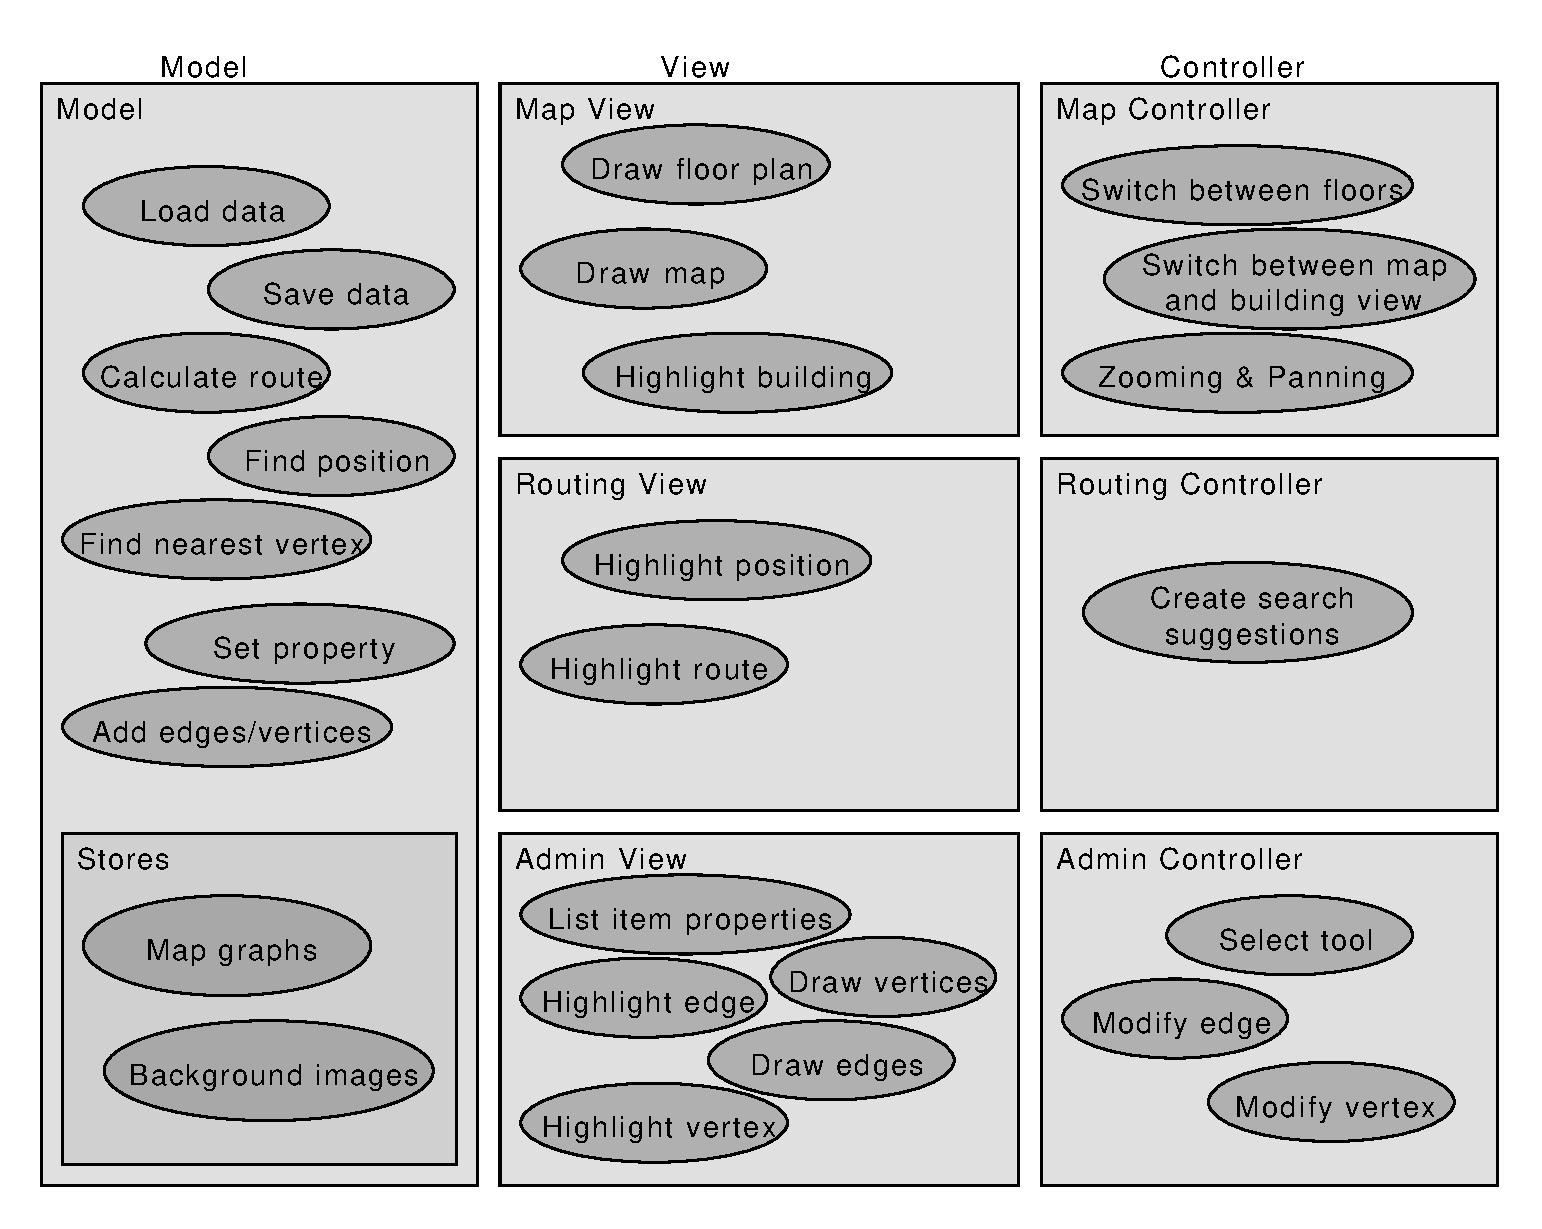
\includegraphics[scale=0.5]{diagrams/mvc.pdf}
	\caption{The parts of the application in the MVC-Architecture}
\end{figure}

The \textit{MVC-architecture} is applied three times inside the project: The map component, the routing tool and the administration tool all use separate views and controllers but share the same model. However, since the routing tool and the administration tool both need to work with the map, they extend the map view and the map controller. \\*
The model has to do the work of the program. It stores the opened \textit{routing graph} and the image that should be displayed as background of the \textit{map} for the exterior and every building floor. It also does the actual routing inside the \textit{routing graph} and offers some functions like finding the nearest vertex for a position. \\*
The view of the map component has to display the currently loaded \textit{map}. This \textit{map} consists of the \textit{background image} either for an interior or an exterior \textit{map}. When the exterior \textit{map} is displayed, a building might be highlighted if one is selected. The routing and administration tools extend this \textit{map} view with their own functionality, for example the routing tool needs a way to display the calculated routes. The administration view shows besides the \textit{map} a panel with the \textit{properties} of the selected edge or vertex.\\*
The controller has to handle the user input. In the case of the map component this means panning and zooming of the \textit{map}, as well as switching between exterior and interior. The controller of the routing tool supports the user to enter his destination since it compares the input with the names of all locations and creates a list of search suggestions. The administration tool controller mainly parses the user input and passes it on to the model to modify the \textit{routing graph}.

\subsection{Use Case Diagram}

\begin{figure}[h]
	\centering
	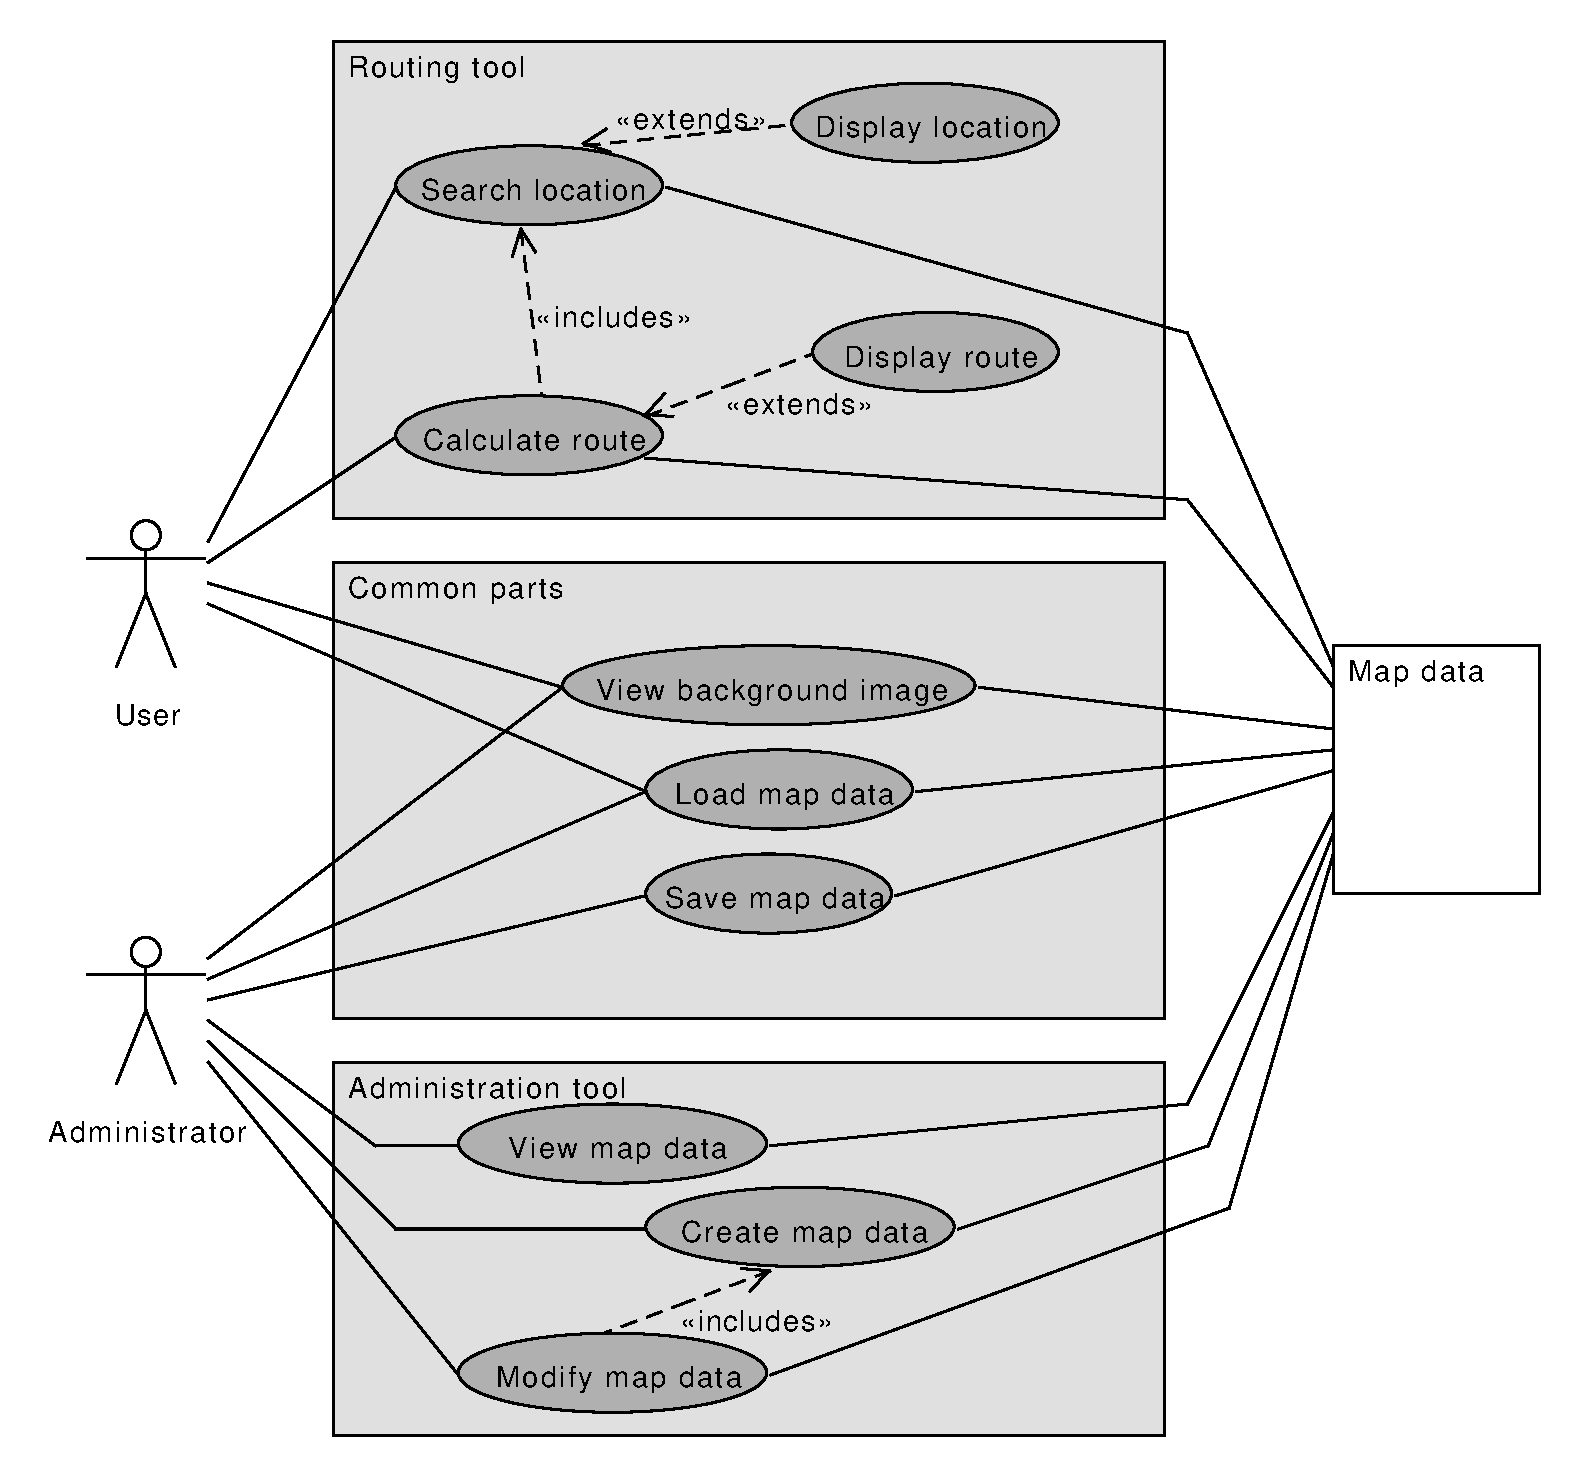
\includegraphics[scale=0.5]{diagrams/usecase.pdf}
	\caption{Possible use-cases of the program}
\end{figure}

After starting the routing tool and loading the \textit{map}, a zoomed out view of the area is displayed. Now the user can look at the \textit{background image} without entering positions. It is possible to zoom into the \textit{map}, move the displayed section and click on buildings to show their floor plan maps. \\*
If he wants to, he can enter a position. This position can be given as coordinates, address, the name of a place or by clicking on the wanted position. By entering only one position, the position will be displayed at the \textit{map} but when he inputs a second position a route between the locations can be calculated and is displayed. The search criteria can be further specified by filtering for some \textit{properties}, for example only stair-free routes can be allowed. \\

To provide this functionality, both program parts needs to have access to the map. This data consists of the \textit{routing graph} that can be modified with the administration tool and the \textit{background image} which has been provided by the user and is linked to the \textit{routing graph}.

\subsection{Activitiy Diagrams}

\subsubsection*{Routing Tool}

\begin{figure}[h]
	\centering
	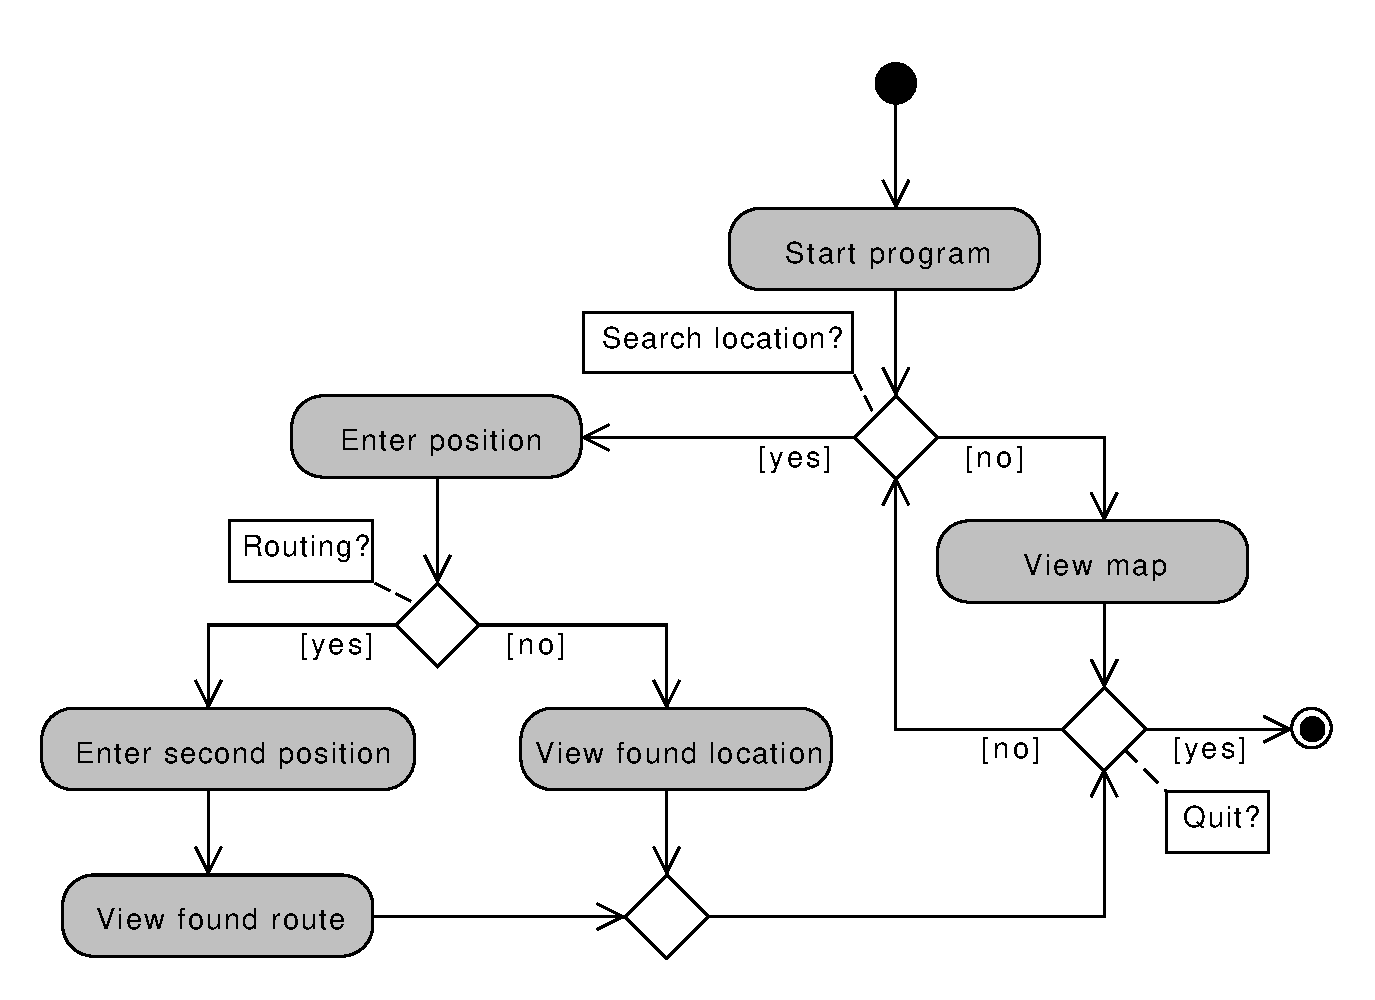
\includegraphics[scale=0.5]{diagrams/activity_routing.pdf}
	\caption{A possible work-flow when using the routing tool}
\end{figure}

The routing tool can be used in three different ways: The user can look at the map, he can search for a location and he can calculate a route between two positions. When he enters a position, the program displays it. After a second position has been entered, the program displays a route between the positions, if one could be found. While calculating this route, the program will follow the restrictions defined by the selected filters. When the user is finished with looking at his route or location, he can either enter new positions or exit the program.

\subsubsection*{Administration Tool}

\begin{figure}[h]
	\centering
	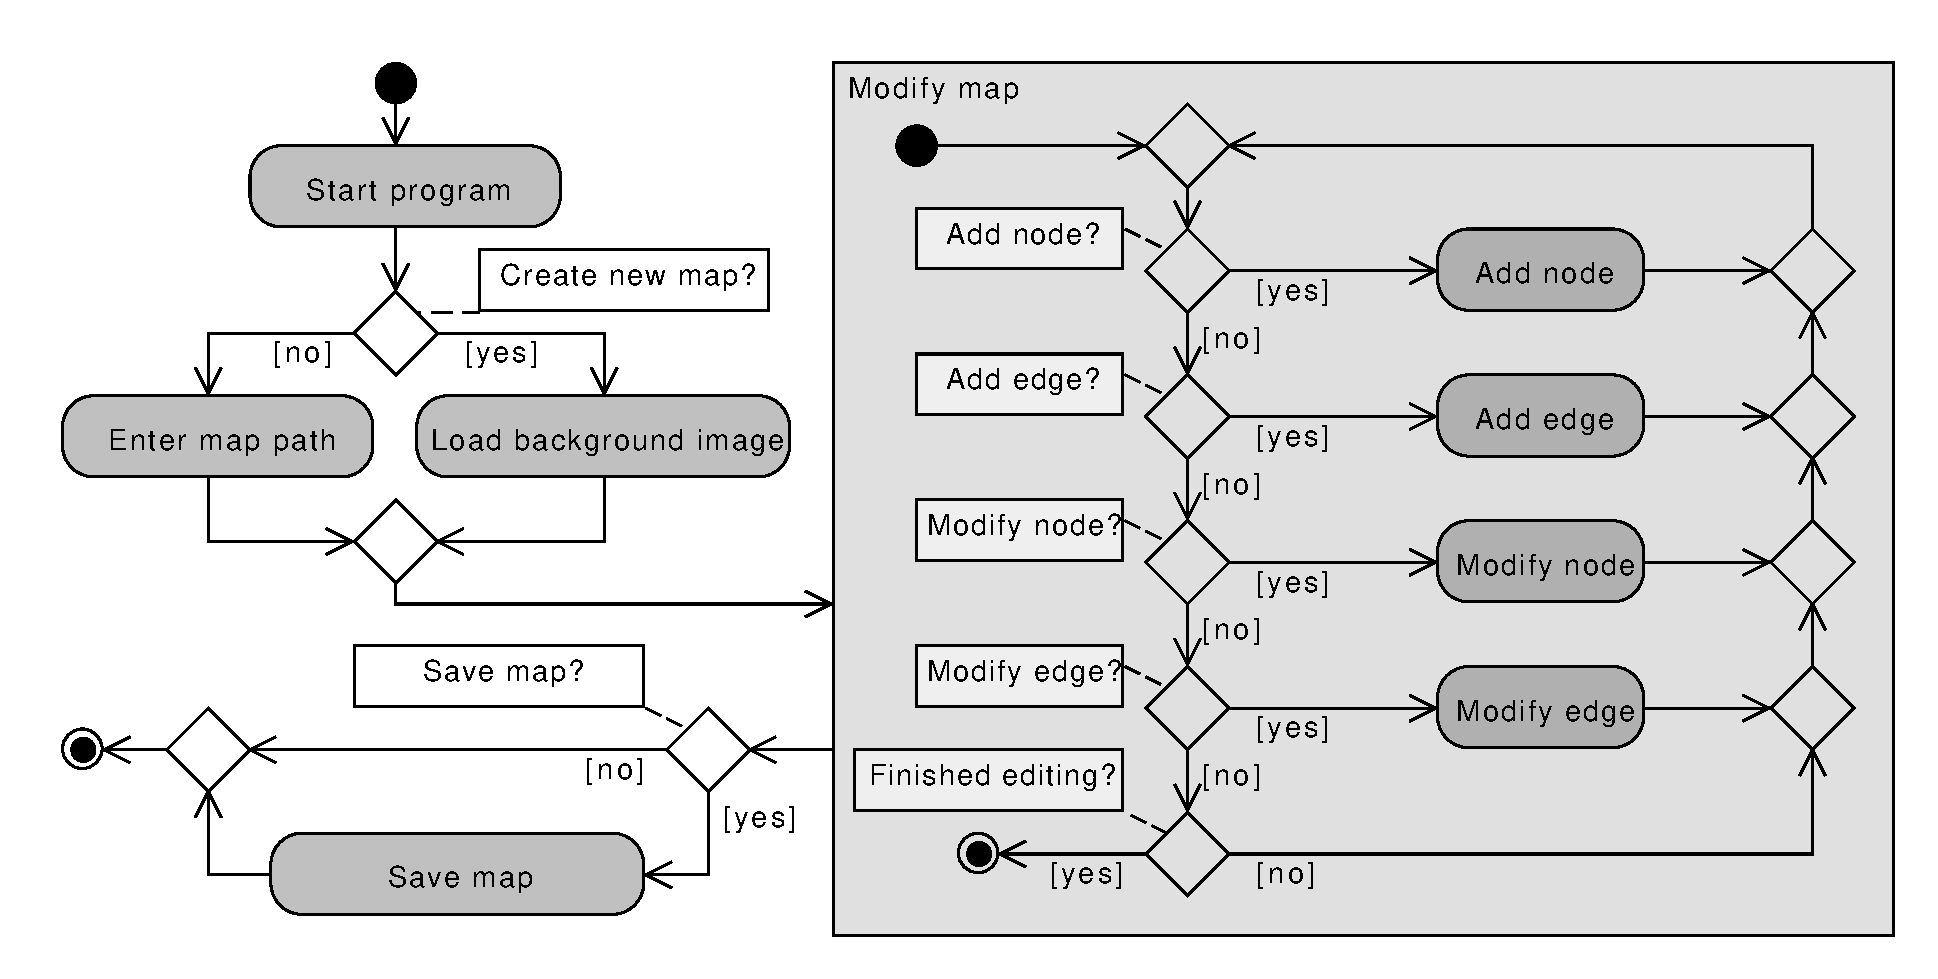
\includegraphics[scale=0.5]{diagrams/activity_admin.pdf}
	\caption{A possible work-flow when using the administration tool}
\end{figure}

The first decision after starting the editor is whether to load an existing map or to load a \textit{background image} to create a new \textit{map}. After doing one of these, the \textit{map} can be modified. To do this the user can add, edit or remove nodes or edges. The \textit{properties} of existing nodes and edges can be edited to attach further information to them, e.g. adding the name of a building to a node. When the user has finished editing the \textit{map}, he can save his changes or drop them if they are not useful.


\newpage
\subsection{Graphical User Interface}
%\subsection{Graphical User Interface}

\subsubsection*{Administration View}
\begin{figure}[!h]
	\centering
	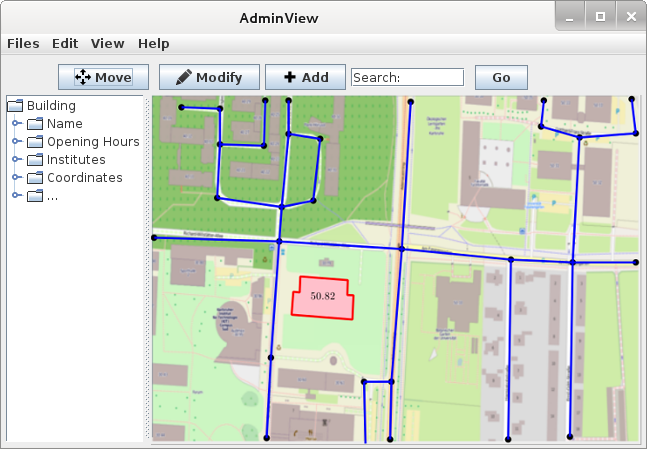
\includegraphics[scale=0.7]{gui-pictures/AdminView.png}
	\caption{Administration view with displayed \textit{routing graph}.}
\end{figure}
The administrator has the option to load and save the \textit{routing graphs} and
background images via the ``Files'' dialogue. In the toolbar below the main menu
will be a collection of tools for modifications of the \textit{routing graph} and
a \textit{search field} for specific locations.
On the right side will be a list of the selected nodes and edges with sub-entries of their
\textit{properties}. The main area shows the editable \textit{routing graph} of the \textit{map} and the \textit{background image}.

\begin{figure}[h!]
\begin{minipage}[hbt]{8cm}
	\centering
	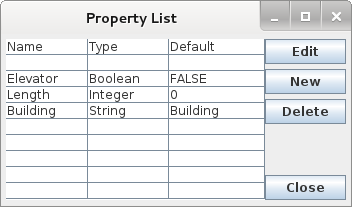
\includegraphics[scale=0.5]{gui-pictures/PropertyList.png}
	\caption{List of configured \textit{properties}.}
        \label{fig:propertyList}
\end{minipage}
\hfill
\begin{minipage}[hbt]{8cm}
	\centering
	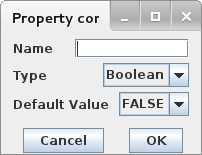
\includegraphics[scale=0.5]{gui-pictures/PropertyConfig.png}
	\caption{Configure a new \textit{property}.}
        \label{fig:propertyConfig}
\end{minipage}
\end{figure}

The \textit{property} list (Figure~\ref{fig:propertyList}) can be accessed through ``Edit --> Properties'' and will show a list of the names, datatypes and default values of
all available \textit{properties}, which can be added to vertices and edges. \\
To edit an entry in this list it has to be selected and then the ``Edit'' button pressed.
To add a new entry to the list the ``New'' button has to be pressed.
In each case a configuration dialogue (Figure~\ref{fig:propertyConfig}) will pop up, where the name, datatype and
default value can be entered.

\begin{figure}[h!]
\begin{minipage}[hbt]{8cm}
	\centering
	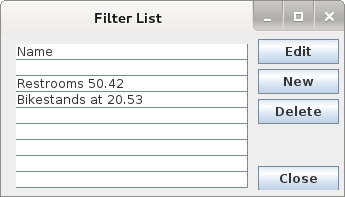
\includegraphics[scale=0.5]{gui-pictures/FilterList.png}
	\caption{List of configured filters.}
        \label{fig:filterList}
\end{minipage}
\hfill
\begin{minipage}[hbt]{8cm}
	\centering
	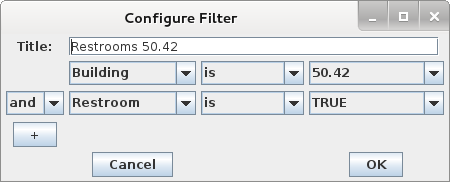
\includegraphics[scale=0.5]{gui-pictures/FilterConfig.png}
	\caption{Configure a filter.}
        \label{fig:filterConfig}
\end{minipage}
\end{figure}

Similar to the \textit{properties} filters will be shown and edited (Figures~\ref{fig:filterList} and~\ref{fig:filterConfig}).

\subsubsection*{Routing View}
\begin{figure}[!h]
	\centering
	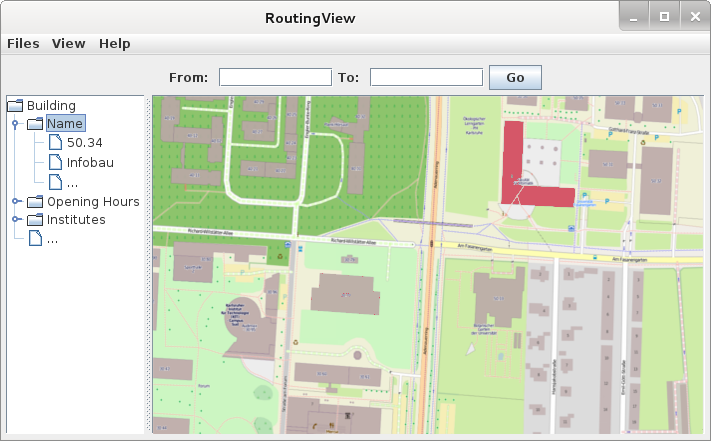
\includegraphics[scale=0.55]{gui-pictures/RoutingView.png} \\
	\caption{Routing view.}
\end{figure}
The routing view has two text fields labeled ``From'' and ``To'' for inserting
the start and endpoint of a route. The main area below shows the \textit{map} and the
calculated path of the route.
On the side of the \textit{map} will be a list of \textit{properties} of the current selection
(building, way, route, etc).

\newpage

\subsubsection*{View inside a building}
\begin{figure}[!h]
	\centering
	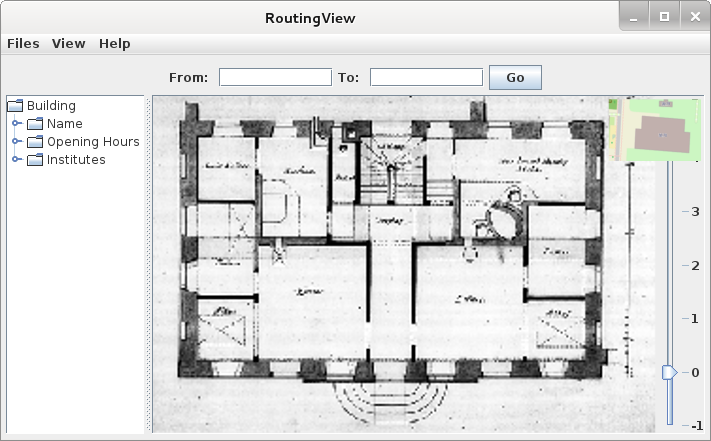
\includegraphics[scale=0.55]{gui-pictures/RoutingView_inside.png} \\
	\caption{Routing view inside a building.}
\end{figure}
The inside view of a building shows the \textit{floor plan map} of a building with an iconized
outside-map in a corner of the main map area. To change the displayed floor a
selection bar will be displayed at the right side.

To enter the building view a building has to be selected while a click on the mini-map or outside the outline of the building exits the building view.


\newpage
\section{Glossary}
\input glossary

\end{document}
